\documentclass{article}

\usepackage[LGR, T1]{fontenc}
\usepackage[utf8]{inputenc}
\usepackage[greek,english]{babel}
\usepackage{alphabeta}
\usepackage{graphicx}
\usepackage{verbatim}
\usepackage{float}

\graphicspath{{../../graphs/session2/}}


\author{Στεφανίδης Ιωάννης}
\title{Δίκτυα Υπολογιστών ΙΙ}
\date{ΑΕΜ: 9587}


\begin{document}

\maketitle

\begin{center}
  \huge Session 2
\end{center}

\section{Echo Packets}

\begin{figure}[H]
  \begin{center}
    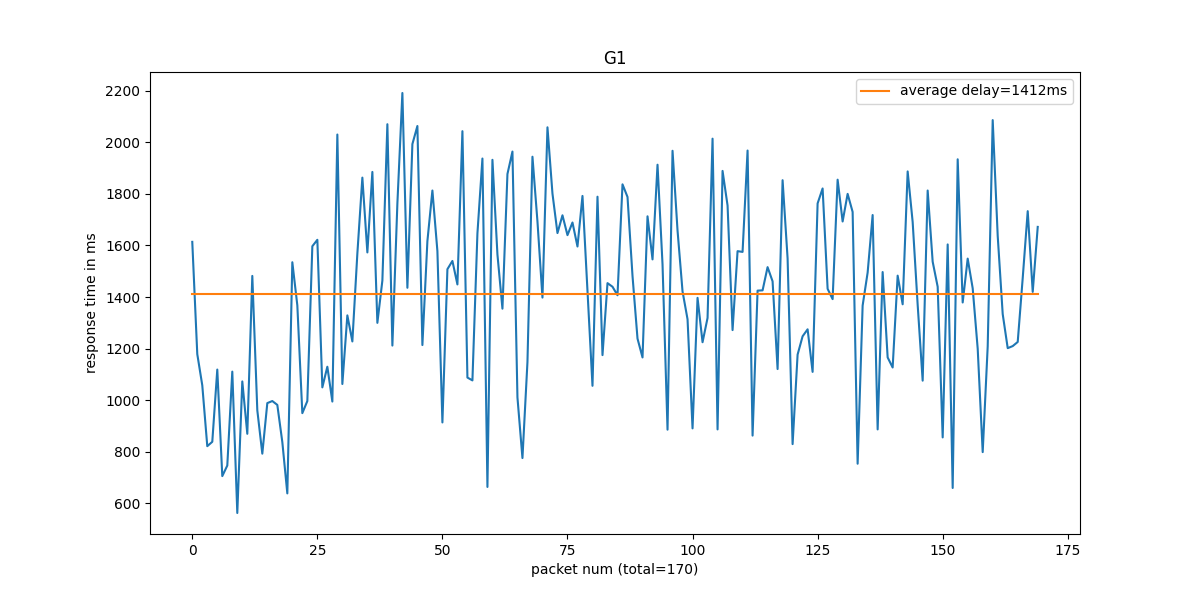
\includegraphics[width=\textwidth]{G1.png}
  \end{center}
  \caption{Χρόνος απόκρισης echo packets με delay για χρονικό διάστημα 4 λεπτά}
\end{figure}

\begin{figure}[H]
  \begin{center}
    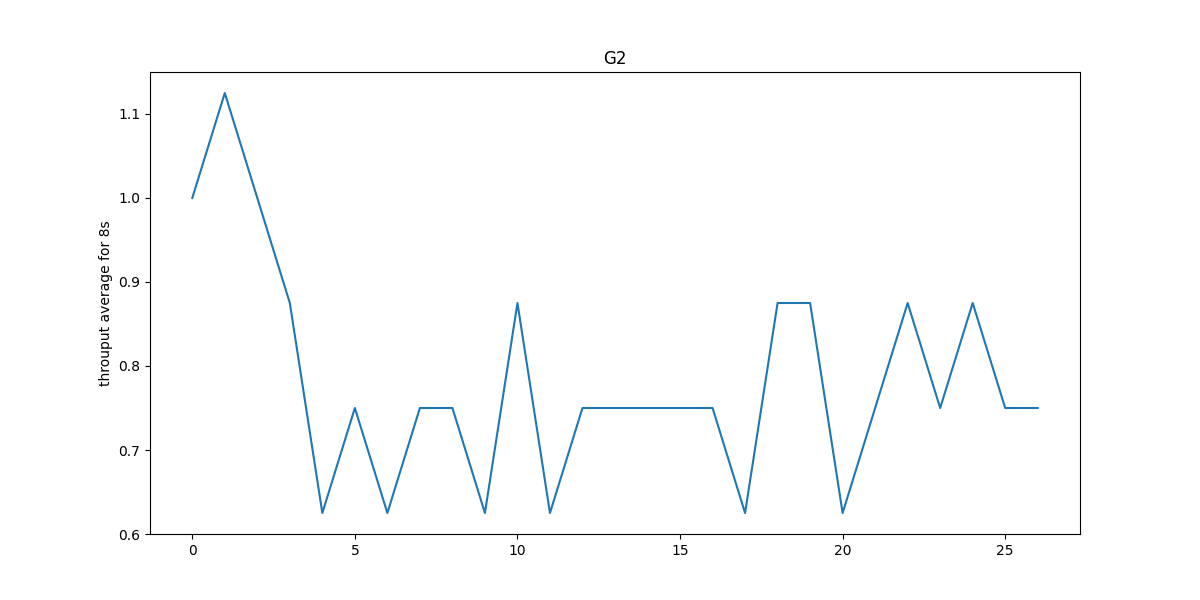
\includegraphics[width=\textwidth]{G2.png}
  \end{center}
  \caption{Throuput echo packets με delay με τεχνική κινούμενου μέσου όρου για 8
  δευτερόλεπτα για χρονικό διάστημα 4 λεπτά}
\end{figure}

\begin{figure}[H]
  \begin{center}
    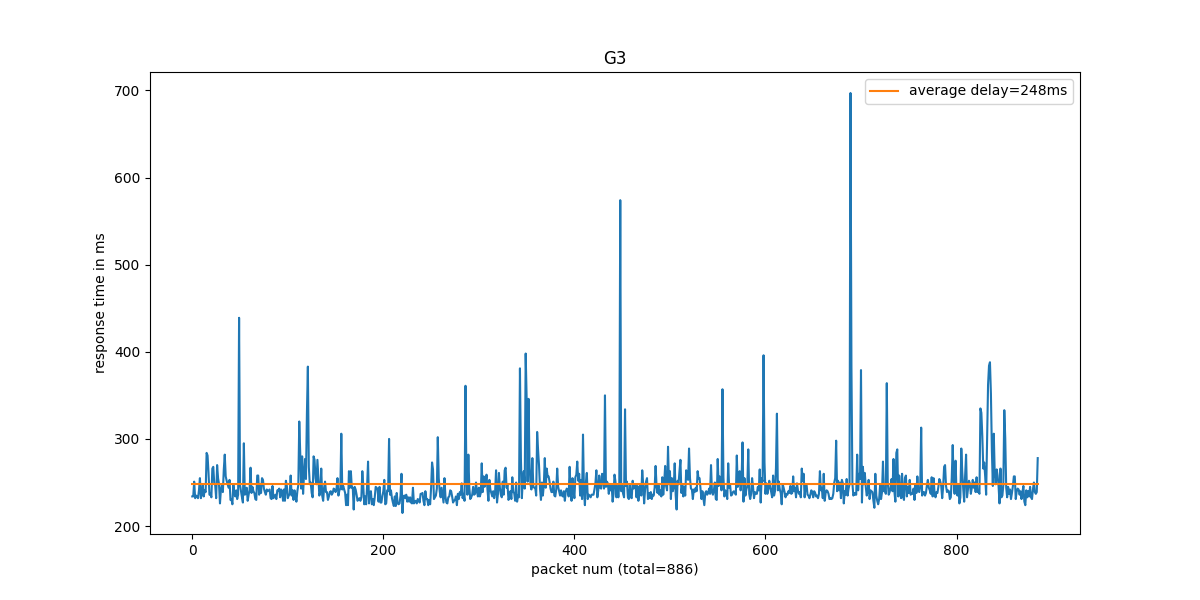
\includegraphics[width=\textwidth]{G3.png}
  \end{center}
  \caption{Χρόνος απόκρισης echo packets χωρίς delay για χρονικό διάστημα 4 λεπτά}
\end{figure}

\begin{figure}[H]
  \begin{center}
    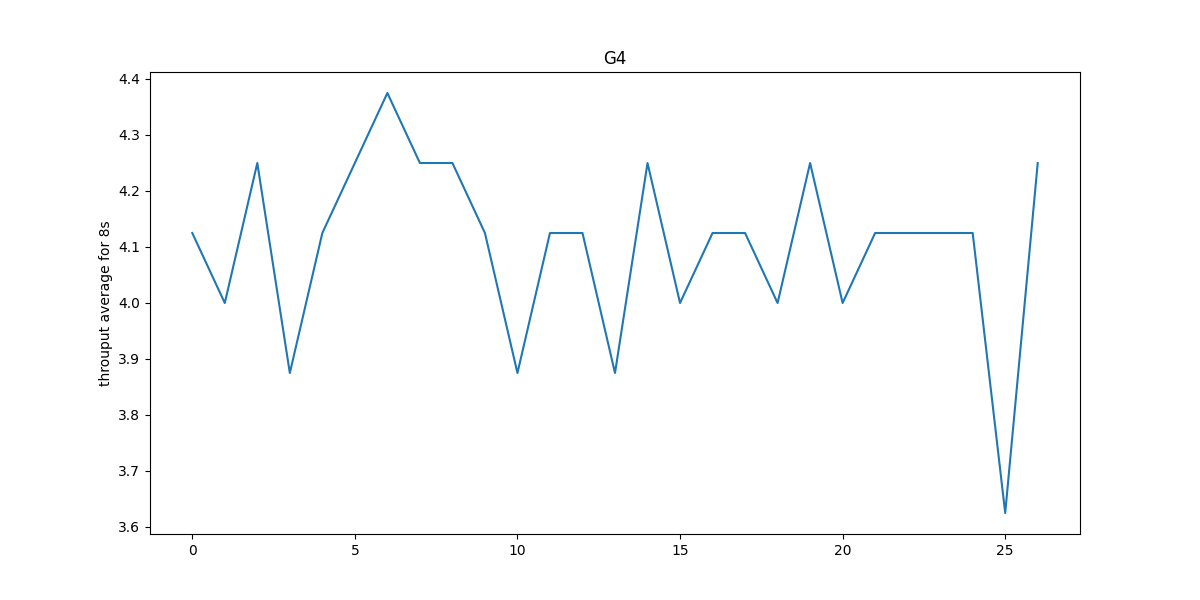
\includegraphics[width=\textwidth]{G4.png}
  \end{center}
  \caption{Throuput echo packets χωρίς delay με τεχνική κινούμενου μέσου όρου για 8
  δευτερόλεπτα για χρονικό διάστημα 4 λεπτά}
\end{figure}

\begin{figure}[H]
  \begin{center}
    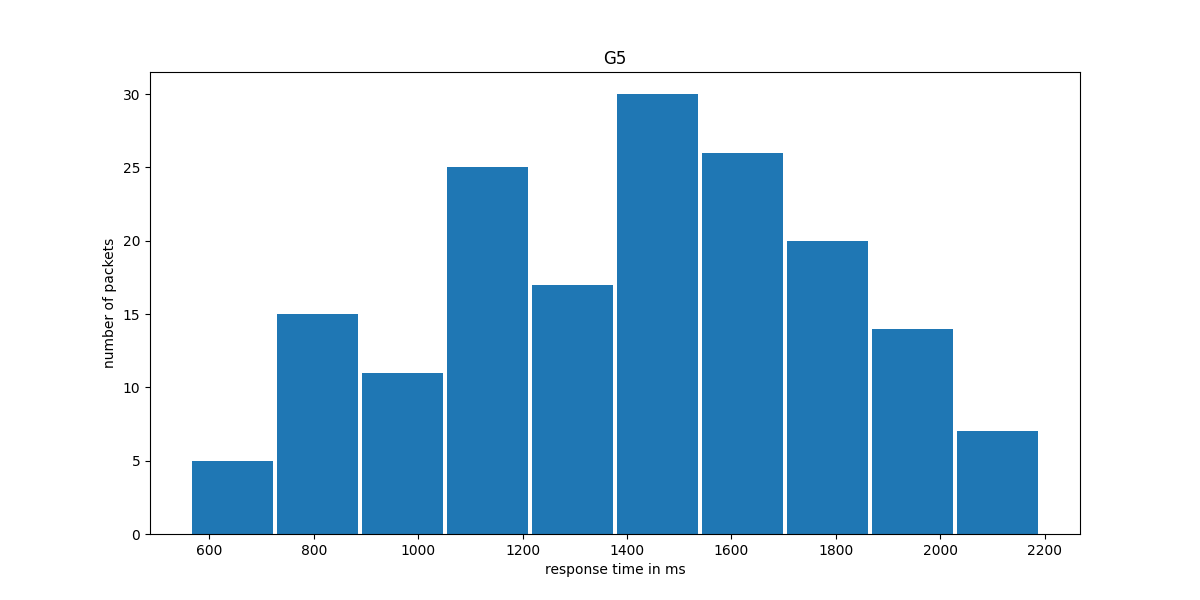
\includegraphics[width=\textwidth]{G5.png}
  \end{center}
  \caption{Ιστόγραμμα χρόνου απόκρισης echo packets με delay για χρονικό διάστημα 4 λεπτά.
  Κανονική κατανομή}
\end{figure}

\begin{figure}[H]
  \begin{center}
    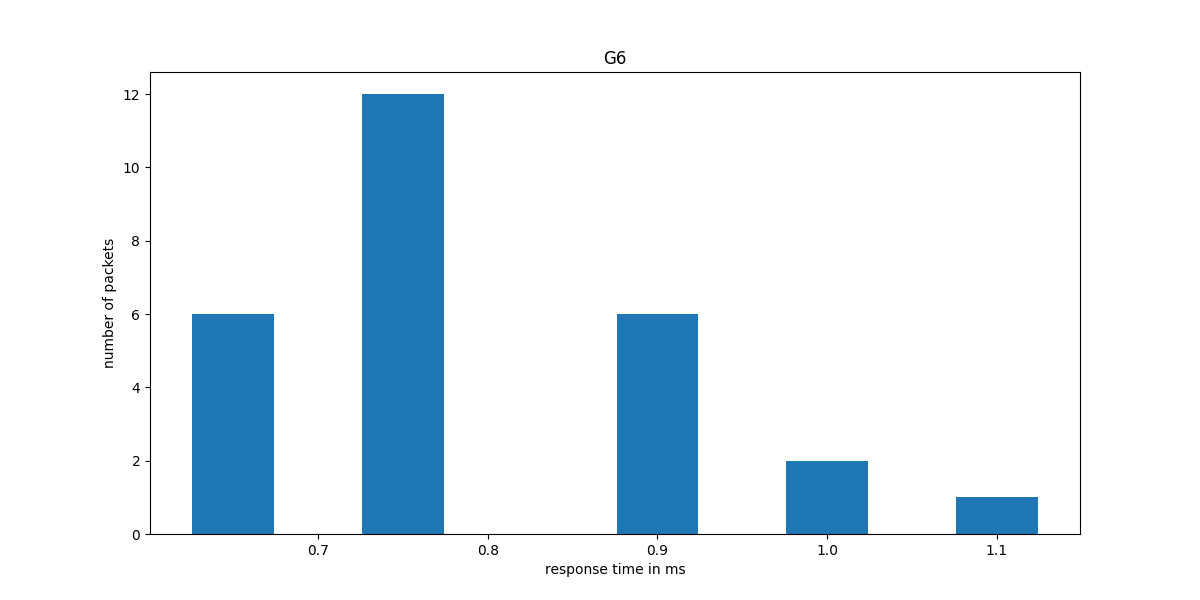
\includegraphics[width=\textwidth]{G6.png}
  \end{center}
  \caption{Ιστόγραμμα throuput echo packets με delay με τεχνική κινούμενου μέσου όρου για 8
  δευτερόλεπτα για χρονικό διάστημα 4 λεπτά}
\end{figure}

\begin{figure}[H]
  \begin{center}
    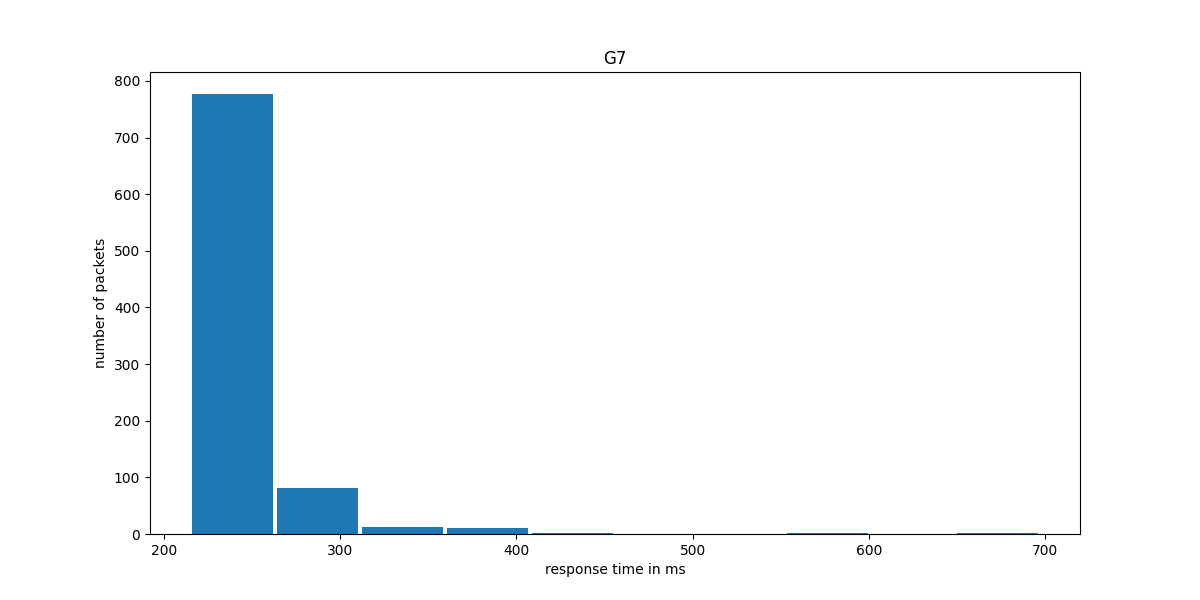
\includegraphics[width=\textwidth]{G7.png}
  \end{center}
  \caption{Ιστόγραμμα χρόνος απόκρισης echo packets χωρίς delay για χρονικό διάστημα 4 λεπτά}
\end{figure}

\begin{figure}[H]
  \begin{center}
    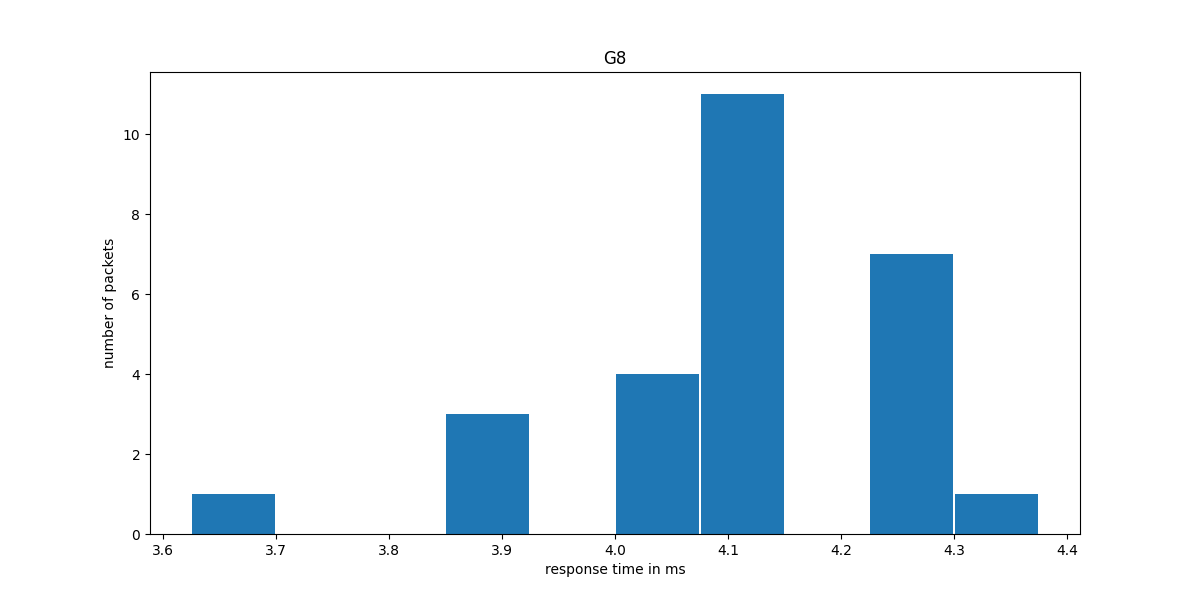
\includegraphics[width=\textwidth]{G8.png}
  \end{center}
  \caption{Ιστόγραμμα throuput echo packets χωρίς delay με τεχνική κινούμενου μέσου όρου για 8
  δευτερόλεπτα για χρονικό διάστημα 4 λεπτά}
\end{figure}

\begin{figure}[H]
  \begin{center}
    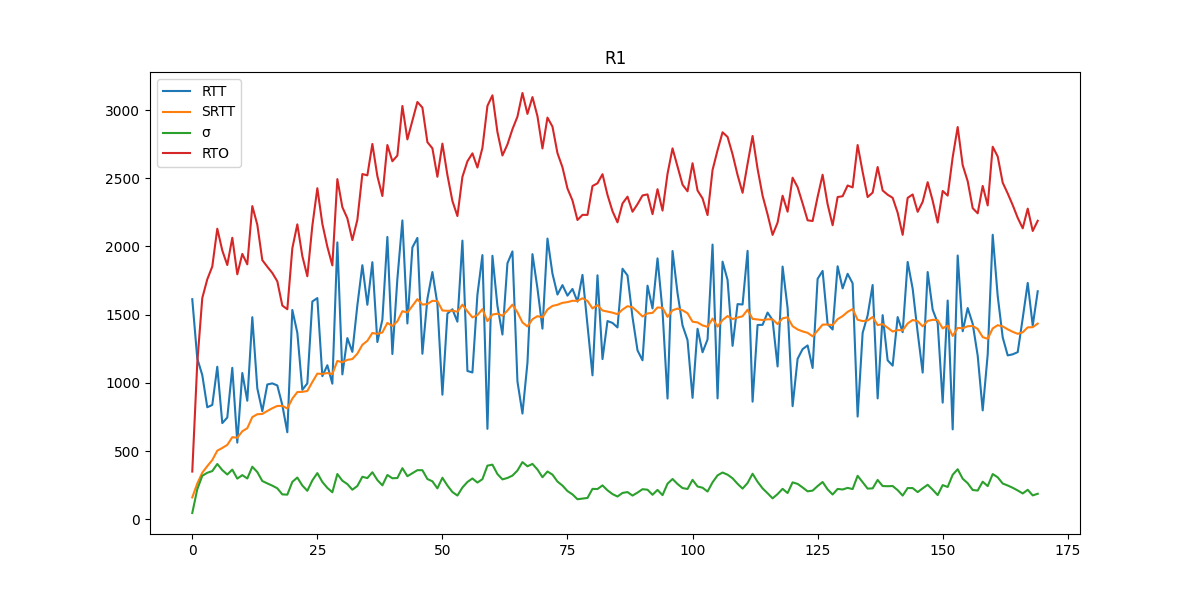
\includegraphics[width=\textwidth]{R1.png}
  \end{center}
  \caption{RTT: Round Trip Time, SRTT: Smooth Round Trip Time, σ{\tiny{RTT}}:
  Round Trip time variance, RTO: Retransmission TimeOut, α=0.9,β=0.8,γ=4}
\end{figure}

\subsection{Temperatures}
\verbatiminput{../../results/session2/E6945_TEMP.txt}

\section{Images}

\begin{figure}[H]
  \begin{center}
    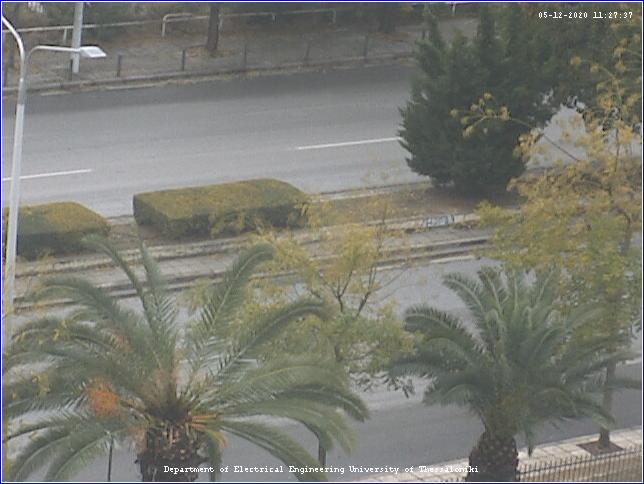
\includegraphics[width=0.8\textwidth]{../../results/session2/E1.jpg}
  \end{center}
  \caption{Εικόνα από την FIX camera}
\end{figure}

\begin{figure}[H]
  \begin{center}
    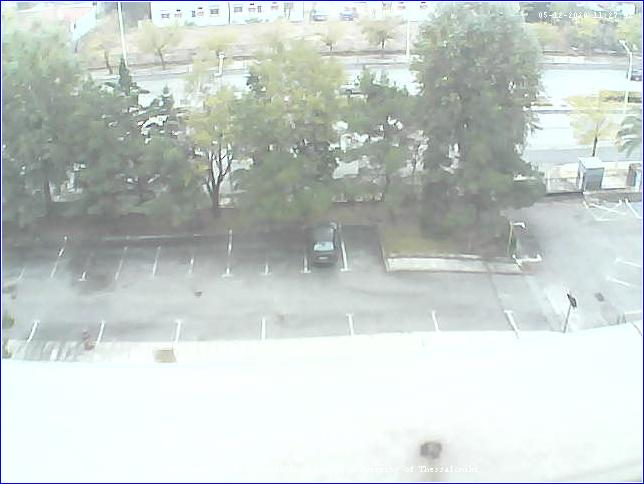
\includegraphics[width=0.8\textwidth]{../../results/session2/E2.jpg}
  \end{center}
  \caption{Εικόνα από την PTZ camera}
\end{figure}

\section{Sound}

\begin{figure}[H]
  \begin{center}
    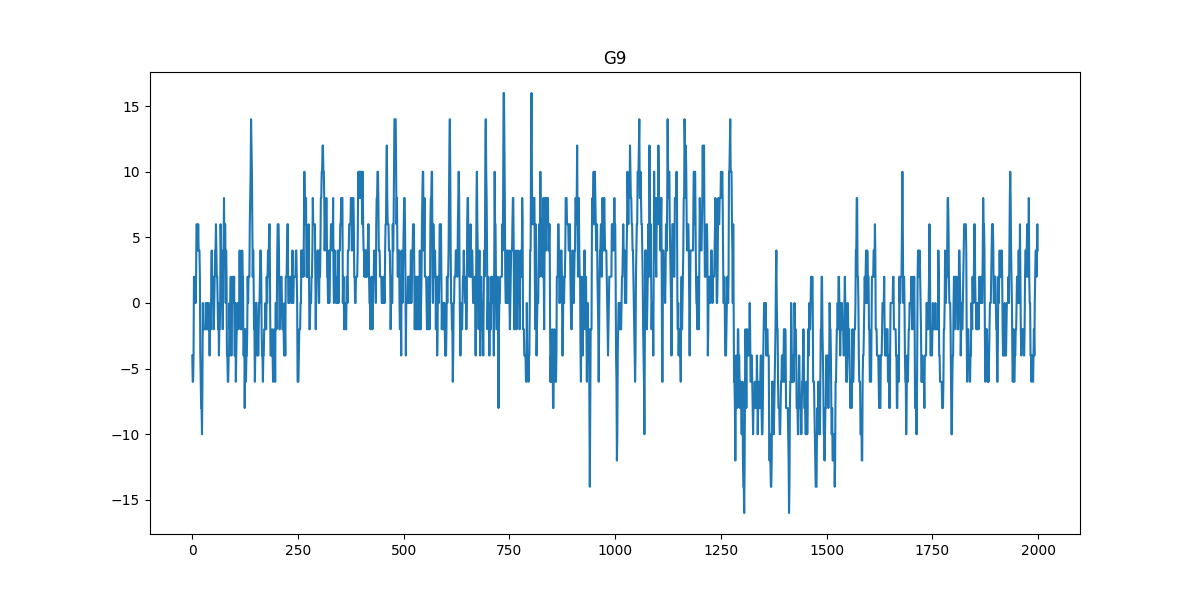
\includegraphics[width=\textwidth]{G9.png}
  \end{center}
  \caption{Τμήμα κυματομορφής τραγουδιού 01 με DPCM}
\end{figure}

\begin{figure}[H]
  \begin{center}
    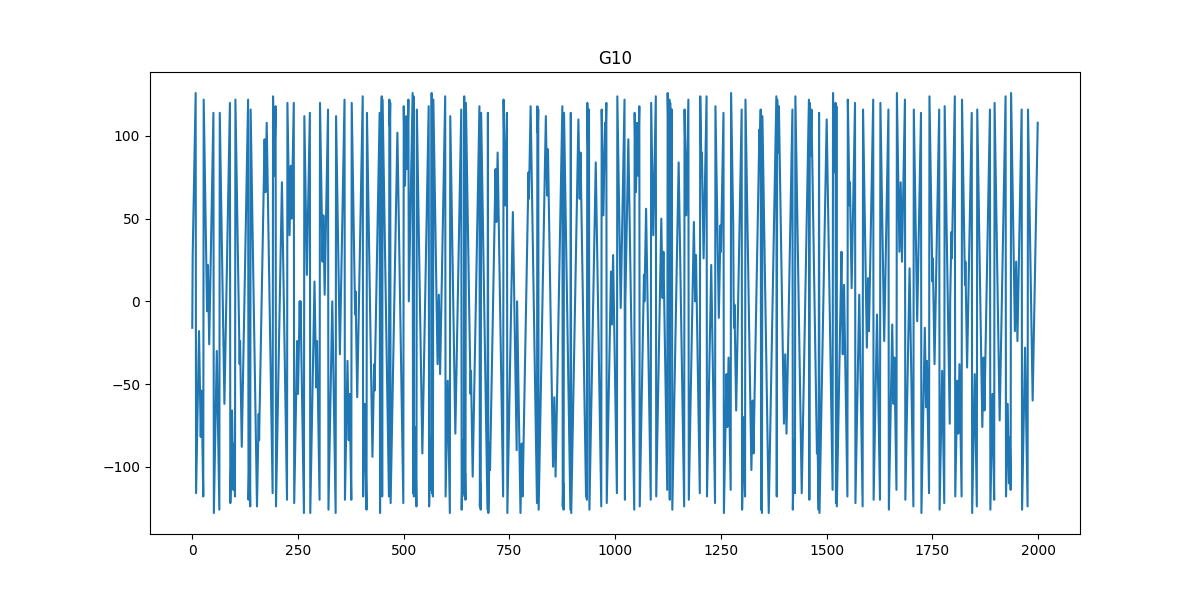
\includegraphics[width=\textwidth]{G10.png}
  \end{center}
  \caption{Τμήμα κυματομορφής εικονικής γεννήτριας με DPCM}
\end{figure}

\begin{figure}[H]
  \begin{center}
    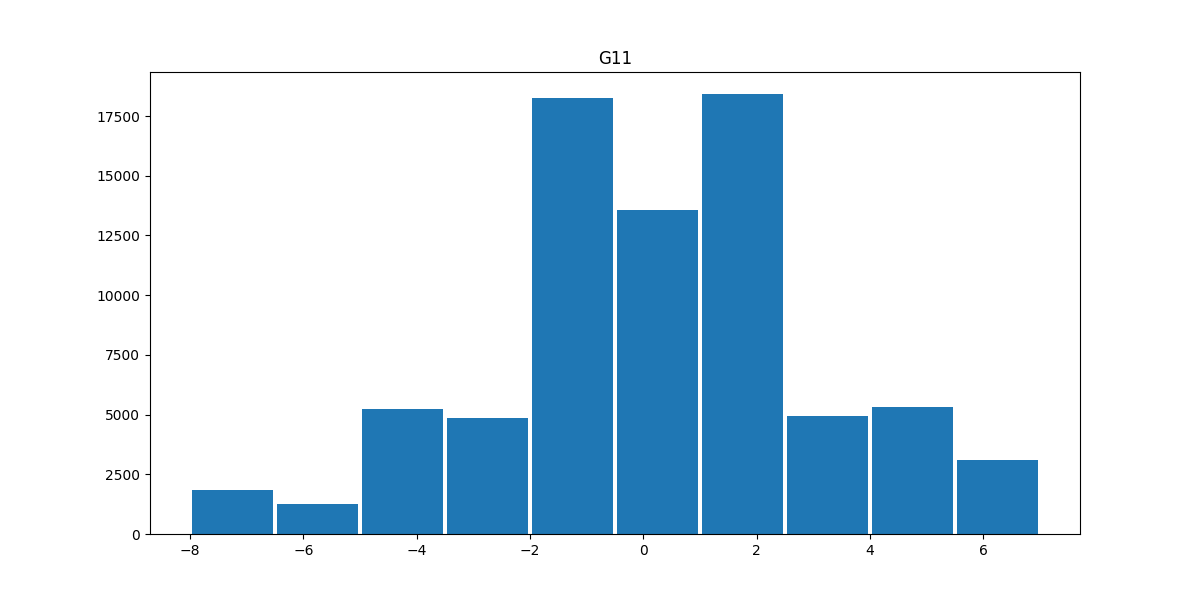
\includegraphics[width=\textwidth]{G11.png}
  \end{center}
  \caption{Ιστόγραμμα διαφορών τραγουδιού 01 με DPCM}
\end{figure}

\begin{figure}[H]
  \begin{center}
    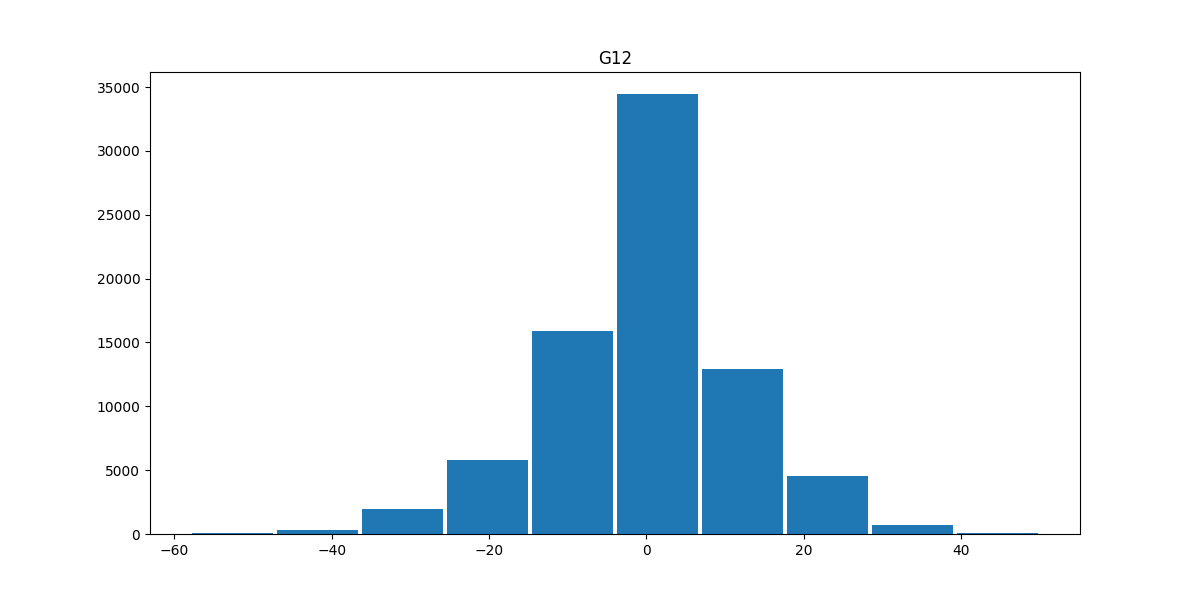
\includegraphics[width=\textwidth]{G12.png}
  \end{center}
  \caption{Ιστόγραμμα δειγμάτων τραγουδιού 01 με DPCM}
\end{figure}

\begin{figure}[H]
  \begin{center}
    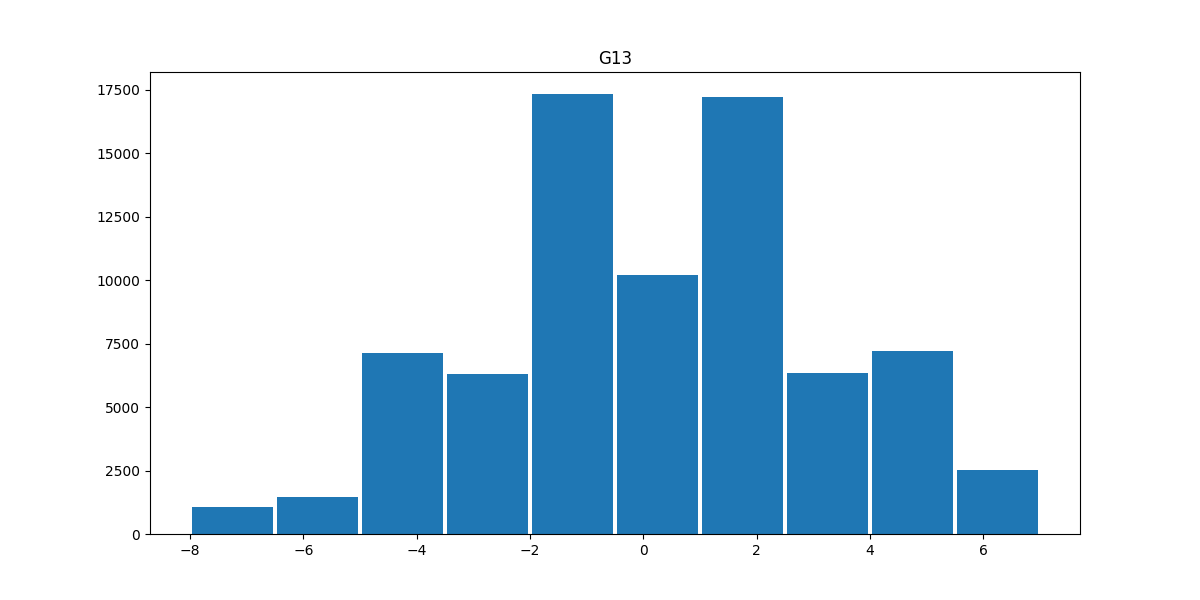
\includegraphics[width=\textwidth]{G13.png}
  \end{center}
  \caption{Ιστόγραμμα διαφορών τραγουδιού 01 με AQ-DPCM}
\end{figure}

\begin{figure}[H]
  \begin{center}
    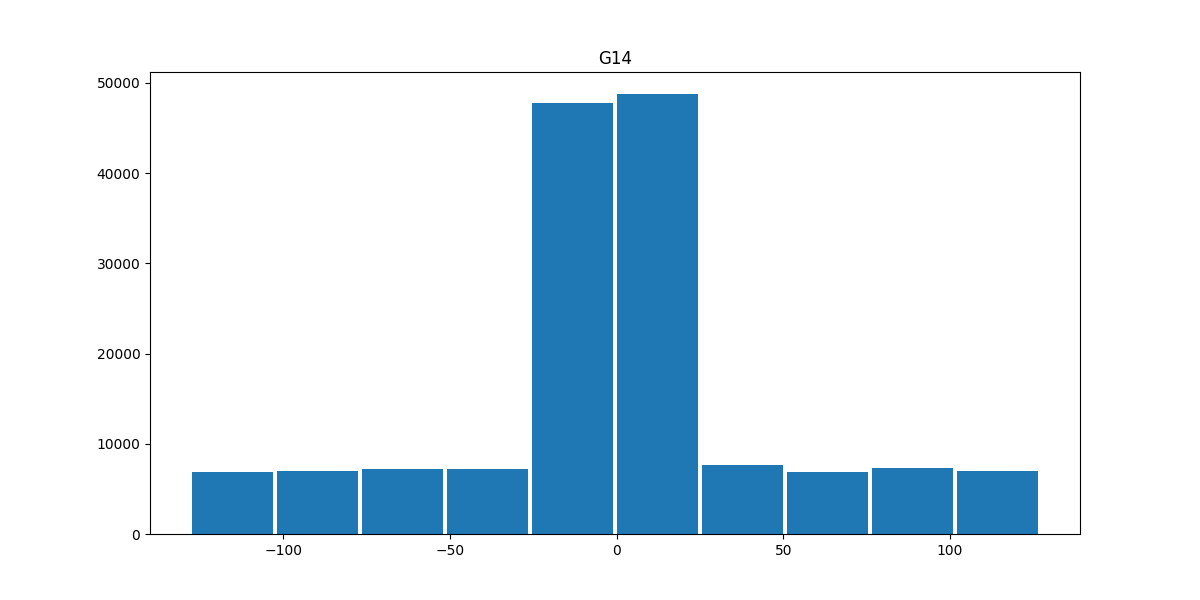
\includegraphics[width=\textwidth]{G14.png}
  \end{center}
  \caption{Ιστόγραμμα δειγμάτων τραγουδιού 01 με AQ-DPCM}
\end{figure}

\begin{figure}[H]
  \begin{center}
    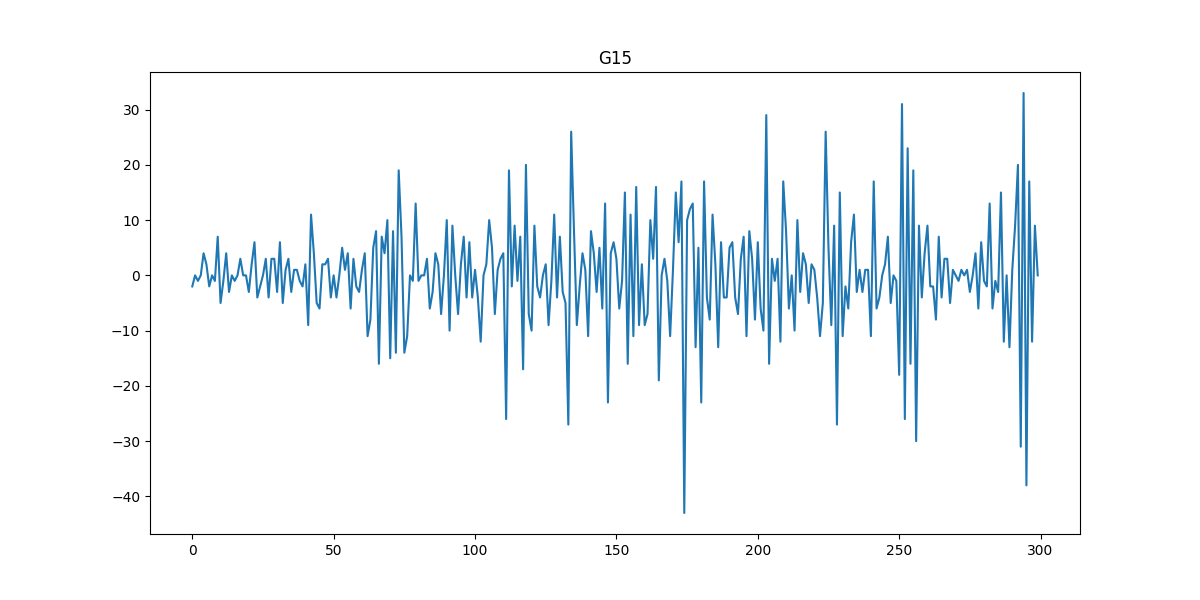
\includegraphics[width=\textwidth]{G15.png}
  \end{center}
  \caption{Διάγραμμα μέσης τιμής τραγουδιού 01 με AQ-DPCM}
\end{figure}

\begin{figure}[H]
  \begin{center}
    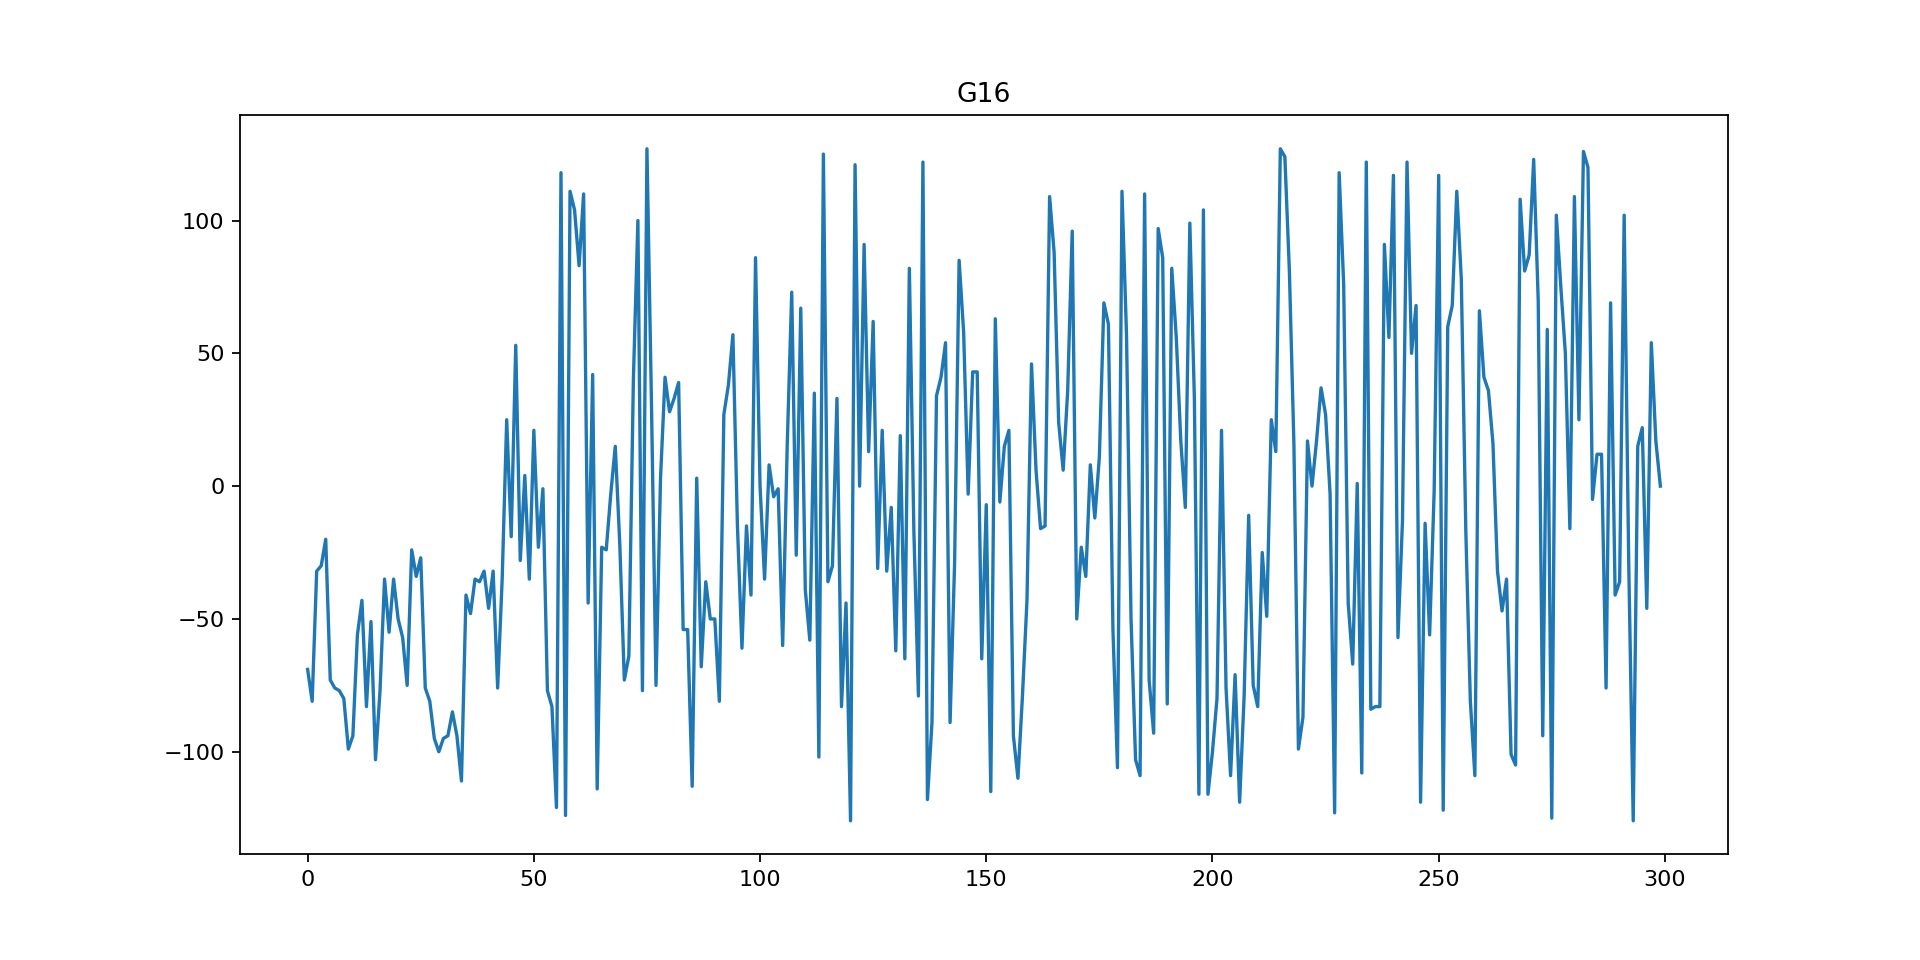
\includegraphics[width=\textwidth]{G16.png}
  \end{center}
  \caption{Διάγραμμα βήματος του προσαρμοσμένου κβαντιστή τραγουδιού 01 με AQ-DPCM}
\end{figure}

\begin{figure}[H]
  \begin{center}
    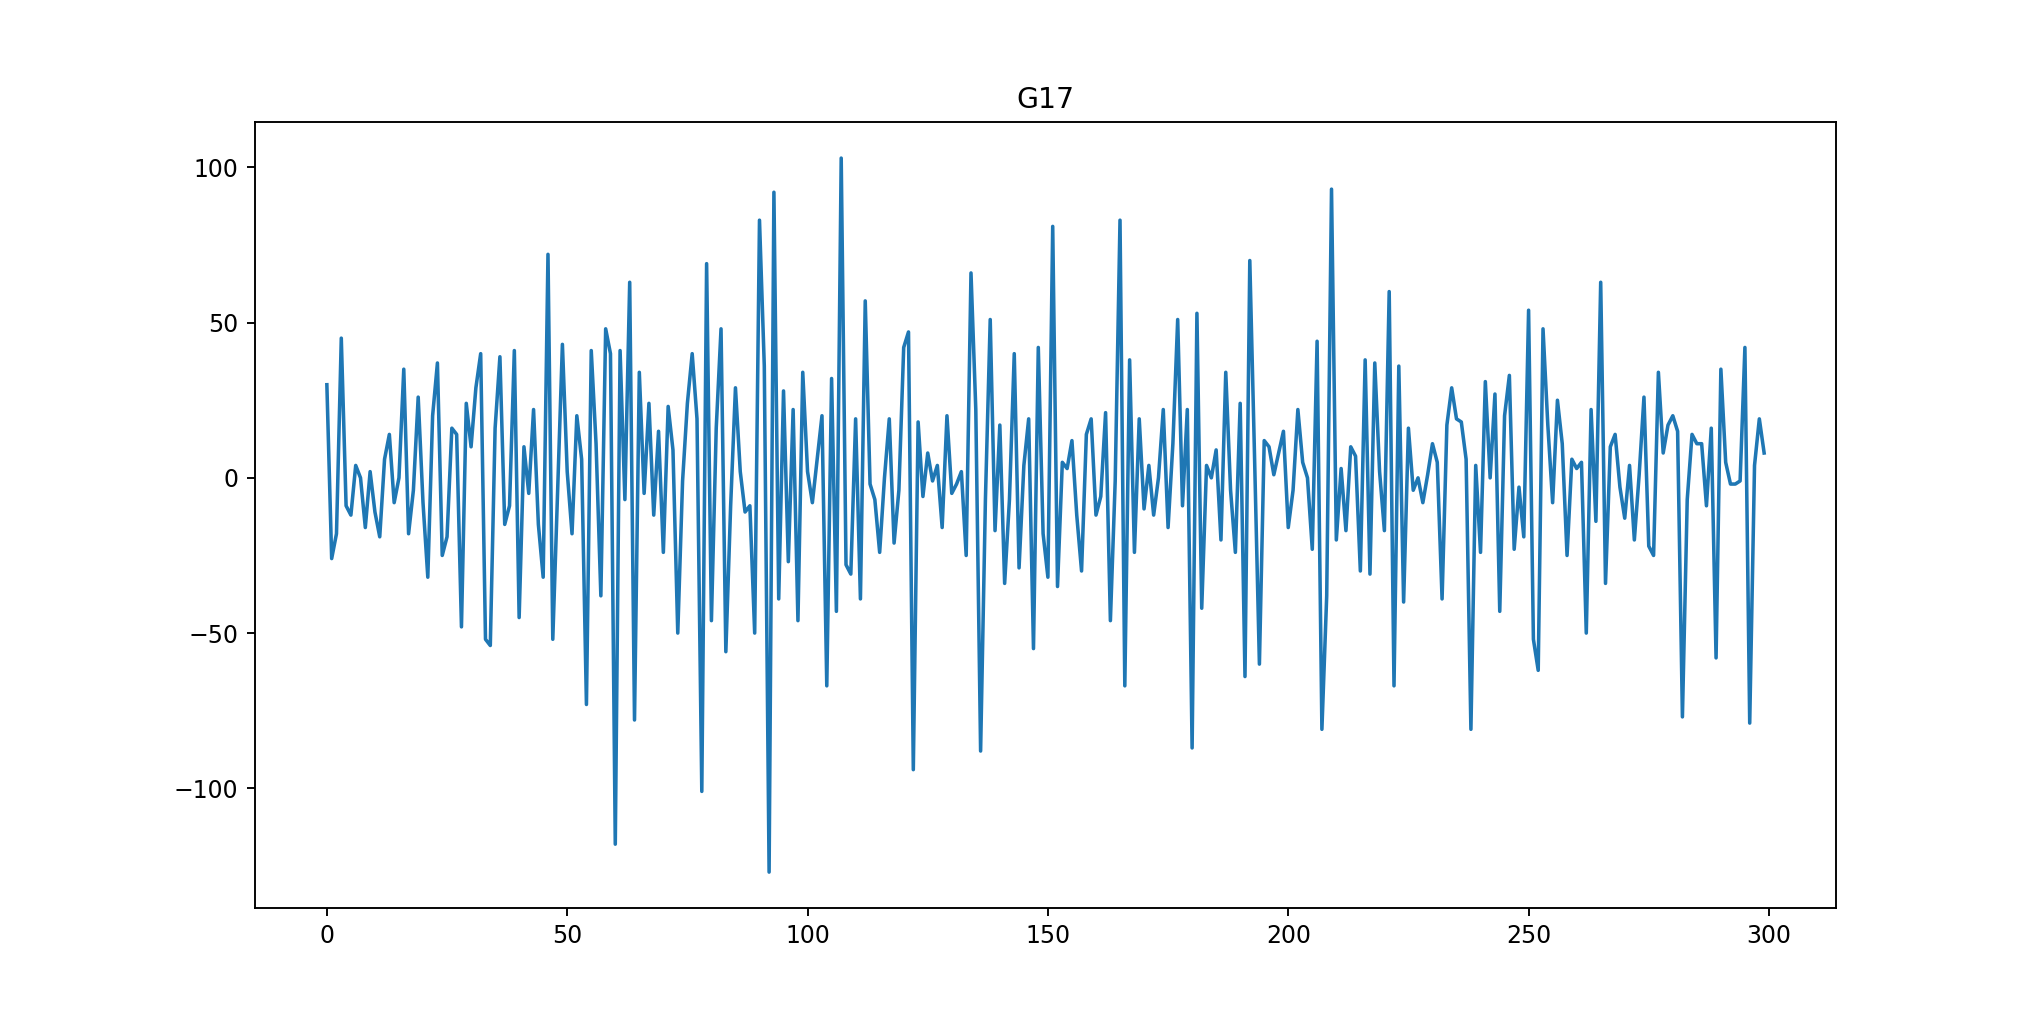
\includegraphics[width=\textwidth]{G17.png}
  \end{center}
  \caption{Διάγραμμα μέσης τιμής τραγουδιού 02 με AQ-DPCM}
\end{figure}

\begin{figure}[H]
  \begin{center}
    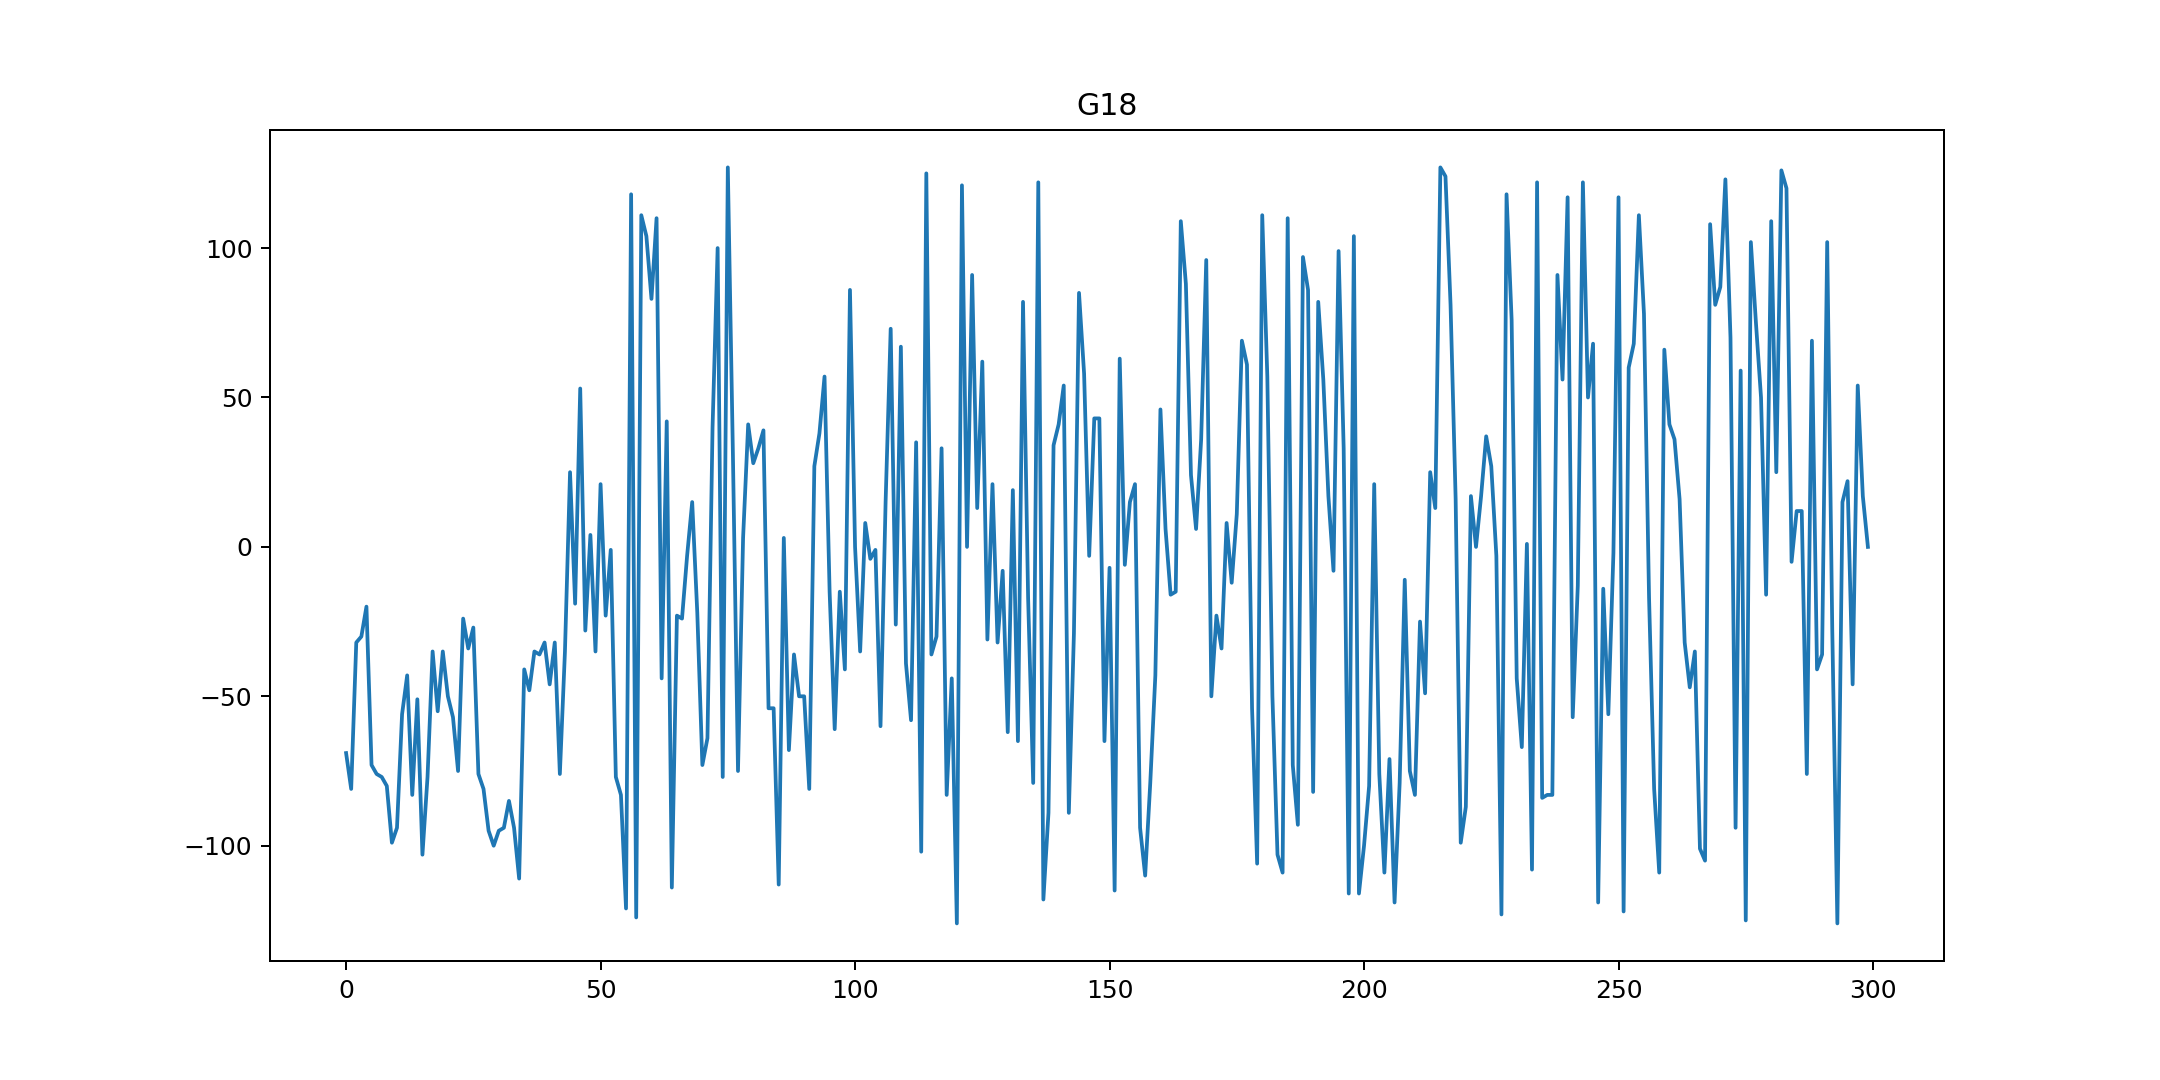
\includegraphics[width=\textwidth]{G18.png}
  \end{center}
  \caption{Διάγραμμα βήματος του προσαρμοσμένου κβαντιστή τραγουδιού 02 με AQ-DPCM}
\end{figure}

\newpage

\section{Ithaki Copter}

\begin{figure}[H]
  \begin{center}
    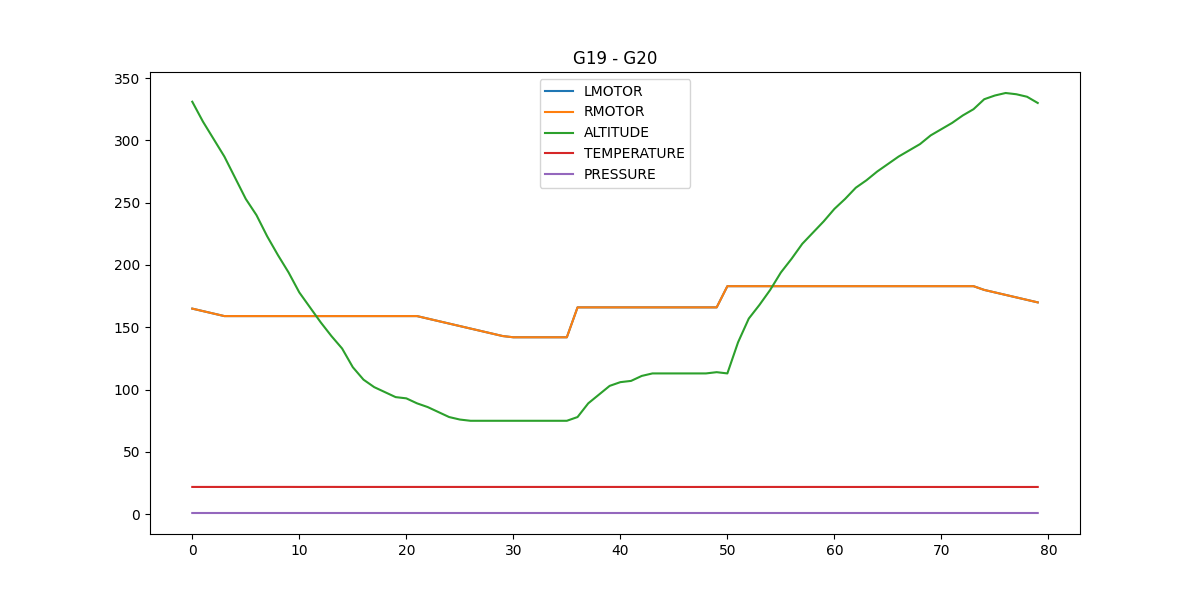
\includegraphics[width=\textwidth]{G19-G20.png}
  \end{center}
  \caption{Διάγραμμα τηλεμετρήσεων από Ithaki Copter για χρονική διάστημα 1 λεπτό}
\end{figure}

\section{Vehicle}

\begin{figure}[H]
  \begin{center}
    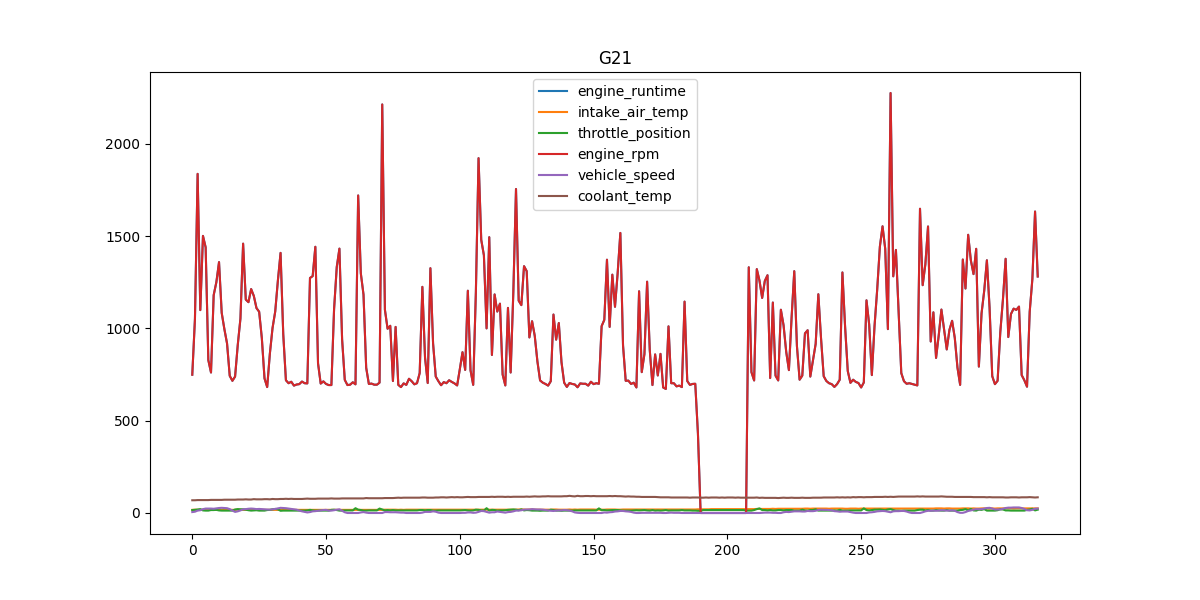
\includegraphics[width=\textwidth]{G21.png}
  \end{center}
  \caption{Διάγραμμα τηλεμετρήσεων από vehicle για χρονική διάστημα 4 λεπτό}
\end{figure}

\section{Session Info}

\subsection{Date}
05/12/2020 11:01

\subsection{Codes used}

\begin{itemize}
  \item E6945
  \item M4748
  \item A6373
  \item V9761
\end{itemize}


\end{document}
